\documentclass{article}

\usepackage[most]{tcolorbox}
\usepackage{physics}
\usepackage{graphicx}
\usepackage{float}
\usepackage{amsmath}
\usepackage{amssymb}


\usepackage[utf8]{inputenc}
\usepackage[a4paper, margin=1in]{geometry} % Controla los márgenes
\usepackage{titling}

\title{Clase 9 }
\author{Manuel Garcia.}
\date{\today}

\renewcommand{\maketitlehooka}{%
  \centering
  \vspace*{0.05cm} % Espacio vertical antes del título
}

\renewcommand{\maketitlehookd}{%
  \vspace*{2cm} % Espacio vertical después de la fecha
}

\newcommand{\caja}[3]{%
  \begin{tcolorbox}[colback=#1!5!white,colframe=#1!25!black,title=#2]
    #3
  \end{tcolorbox}%
}

\begin{document}
\maketitle

\section{Series y convergencia}
En la clase pasada demostramos que $ \sum_{n = 0 }^{\infty}|a_n|<\infty \leftarrow  \rightarrow \sum_{n=0 }^{\infty}a_n  $: converge. 
\begin{gather*}
  S_n = a_0+a_1+a_2+...+a_n \\
  v_n = \left|a_0 \right|+\left|a_1 \right| + \left|a_2 \right|+...+\left|a_n \right|\\
  n>m\geq N \\
  \left|S_n - S_m \right| = \left|\displaystyle\sum_{j = m+1 }^{\infty}a_j \right| \geq \displaystyle\sum_{j = m+1 }^{\infty}\left|a_j \right| = v_n - v_m \\
  \text{Como la cola converge demostramos que la serie tambien converge.}
\end{gather*}

\subsection{Algunos criterios de convergencia }
\begin{itemize}
  \item Criterio de la comparación: 

    Supongamos que $ a_n  $ son números complejos y $ b_n  $ son numeros reales, si para todo $ n \geq n_n  $
    \begin{gather*}
      \left|a_n \right|\leq b_n \qquad y \qquad \displaystyle\sum_{n= 0 }^{\infty}b_n  
    \end{gather*}
    Es convergente, entonces $ \displaystyle\sum_{n = 0 }^{\infty}a_n  $ es convergente 
    \begin{gather*}
      \text{\textbf{Ejemplo }}\\
      \displaystyle\sum_{n = 0 }^{\infty} \frac{2 e ^ {i n }}{n ^2 + 3 } = \left|\frac{2 e ^ {in }}{n ^2 + 3 }\right| = \frac{2 }{n ^2 + 3 }<\frac{2 }{n ^2} \\
      \text{Por el criterio de comparacion el modulo de esta cantidad siempre va a estar acotado }\\
      \text{Como }\displaystyle\sum_{n = 1 }^{\infty} \frac{2 }{n ^2} \text{ converge }\rightarrow \qquad \displaystyle\sum_{n = 0 }^{\infty}\frac{2 e ^ {in }}{n ^2 + 3 }: \text{ Converge}
    \end{gather*}
  
  \item Prueba de la razon 
    \begin{gather*}
      p = \underset{n \rightarrow \infty}{lim }\left|\frac{a _{n + 1 } }{a_n } \right|, \qquad  \\
      \text{Si }p<1\text{ entonces la serie }\displaystyle\sum_{n = 0 }^{\infty}a_n \quad \text{Converge absolutamente y diverge si }p>1\\
      \text{En el caso en que }p=1 \text{ no se puede afirmar algo}
    \end{gather*}
    \begin{gather*}
      \text{\textbf{Ejemplo }}\\
      \displaystyle\sum_{n = 0 }^{\infty} \frac{z ^ {n }}{n! } = \underset{n \rightarrow \infty}{lim }\left|\frac{\frac{z ^ {n+ 1 }}{(n+1)! }}{\frac{z^n }{n! }}\right| = \underset{n \rightarrow \infty}{lim} \frac{\left|z \right|}{n+1 } = 0\\
      \text{Es convergente ya que }p<1
    \end{gather*}
\end{itemize}

\caja{green}{Definicion }{
  $ \sum_{n = 0 }^{\infty}a_n, \quad \sum_{n = 0 }^{\infty}b_n  $ ambas series de Cauchy 
  \begin{gather*}
    \displaystyle\sum_{n = 0 }^{\infty}c_n  = \left(\displaystyle\sum_{n = 0 }^{\infty}a_n \right)\left(\displaystyle\sum_{n = 0 }^{\infty}b_n \right) 
  \end{gather*}
}

\subsection{Funciones elementales de la variable compleja }
\begin{gather*}
  f\left(z\right)=e ^ {z }\\
  e ^ {x } = \displaystyle\sum_{n = 0 }^{\infty} \frac{x ^ {n }}{n! }\\
  e ^ {\left|z \right|} = \displaystyle\sum_{n = 0 }^{\infty} \frac{\left|z \right|^ {n }}{n! }, \qquad e ^ {z } =  \displaystyle\sum_{n = 0 }^{\infty} \frac{z ^ {n }}{n! }
\end{gather*}
Si $ z = i \theta  $
\begin{gather*}
  e ^ {i \theta } = \displaystyle\sum_{n = 0 }^{\infty} \frac{(i\theta )^ {n }}{n! }\\
  = \displaystyle\sum_{n = 0 }^{\infty} (-1 )^ {n }\frac{\theta ^ {2n }}{(2n)! } + i \displaystyle\sum_{n = 0 }^{\infty}(-n )^ {n }\frac{\theta ^ {2n + 1 }}{(2n+1)! }\\
  \cos{\theta} = \displaystyle\sum_{n = 0 }^{\infty}(-1)^ {n } \frac{\theta ^ {2n }}{(2n)! }, \qquad \qquad \sin{\theta} = \displaystyle\sum_{n = 0 }^{\infty}(-1)^ {n }\frac{\theta ^ {2n + 1 }}{(2n + 1)!}
\end{gather*}

\textbf{Ejemplo } Vamos a levar un dominio de un rectangulo entre $ A = (-2,0 ),\quad B = (-2,2),\quad C = (2,2,),\quad D = (2,0) $ al plano comlejo con la funcion $ f\left(z\right)=e ^ {z } = e ^ {x + i y } $. 

Para $ A  $
\begin{gather*}
  u = e ^ {x }\cos{y }, \qquad v = e ^ {x }\sin{y }\\
  A(-2,0) \quad \rightarrow \quad A'(e ^ {-2 }, 0 ) \\
  B(-2,2) \quad \rightarrow \quad B' (e ^ {-2 }\cos{2 }, e ^ {-2 }\cos{2 })\\
  C(2,2) \quad \rightarrow \quad C'(e ^ {2 }\cos{2 }, e ^ {2 }\sin{2 })\\
  D(2,0 ) \quad \rightarrow \quad D'(e ^ {2 }, 0)
\end{gather*}
\begin{figure}[H]
  \begin{center}
    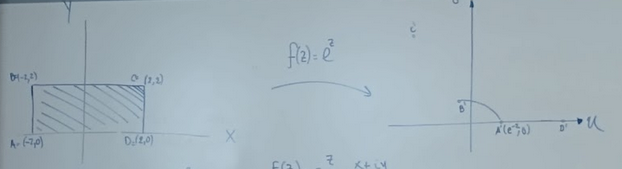
\includegraphics[width=0.8\textwidth]{transformacion_dominio_ej1.png}
  \end{center}
\end{figure}

\hfill

Como transforman las lineas? 

\begin{gather*}
  A-B \\
  x = - 2, \qquad 0\leq y \leq 2 \\
  u ^2 + v ^2 = e ^ {2x } \quad \rightarrow \quad u ^2 + v ^2 = e ^ {-4} \\
  \tan{y } = \frac{v }{u }\\
  B-C \\
  -2 \leq x \leq 2, \qquad y = 2\\
  \tan{2 } = \frac{v }{u }\quad \rightarrow \quad v = u \tan{2 }\\
  C- D \\
  x = 2 \qquad 0 \leq y \leq 2 , \qquad v ^2 + u ^2 = e ^ {4 }\\
  D-A \\
  -2 \leq x \leq 2 , \qquad y = 0 \\
  \tan{0 } = \frac{v }{y } = 0 \quad \rightarrow \quad v = 0 
\end{gather*}

\caja{red}{Seno y coseno }{
  \begin{gather*}
    \cos{z } = \frac{e ^ {i z } + e ^ {i z }}{2 } \qquad \qquad \sin{z } =  \frac{e ^ {i z } - e ^ {i z }}{2i } 
  \end{gather*}
}

Queremos transformar la region dentro del cuadrado $ (0,0),(2,0),(1,2),(0,1 ) $ con la funcion $ f\left(z\right)=\sin{z } $.
\begin{gather*}
  \sin{x+iy } = \frac{e ^ {i (x+ i y )} - e ^ {i (x+iy )}}{2i } = \frac{e ^ {ix }e ^ {-y } - e ^ {-ix }e ^ {y }}{2i} = \frac{(\cos{x }+ i \sin{x }) e ^ {-y }- (\cos{x } - i \sin{x }) e ^ {y }}{2i }\\
  = -\frac{i }{2}\left[(\cos{x } + i \sin{x })e ^ {-y } - (\cos{x } - i \sin{x })e ^ {y }\right]\\
  = \frac{- i e ^ {-y }\cos{x } + e ^ {-y } \sin{x } + i e ^ {y }\cos{x } +  e ^ {y } \sin{x }}{2}\\
  = u + i v \\
  u = \frac{e ^ {-y }\sin{x } + e ^ {y }\sin{x }}{2} = \cosh{y}\sin{x}, \qquad v  = \frac{-e ^ {-y }\cos{x } + e ^ {y }\sin{x }}{2} = \sinh{y}\cos{x}
\end{gather*}
Entonces para clacular las lineas: 
\begin{gather*}
  A-B: x = 0, \quad 0 \leq y \leq 2 \\
  u = \cosh{y }\sin{0 } = 0, \quad u = 0. \quad \qquad v = \sinh y \cos{0 } = \sinh y , \quad 0 \leq v \leq \sinh 2\\
  B-C: 0 \leq x \leq 1, \quad y = 2 \\
  u = \cosh 2 \sin{x } \qquad \qquad v = \sinh 2 \cos{x }\\
  \left(\frac{u }{\cosh 2 }\right)^2 + \left(\frac{v }{\sinh 2 }\right)^2 = 1\\
  C-D: x = 1, \quad 0 \leq y\leq 2\\
  u = 
\end{gather*}
\caja{black}{}{
\textbf{Terminar ejercicio para la proxima clase}
}

\end{document}
